\documentclass[conference]{IEEEtran}
\IEEEoverridecommandlockouts
\pdfminorversion=7
\pdfcompresslevel=0
\pdfobjcompresslevel=0

\usepackage{cite}
\usepackage{amsmath,amssymb}
\let\proof\relax
\let\endproof\relax
\usepackage{amsthm}
\usepackage{graphicx}
\usepackage{booktabs}
\usepackage{array}
\usepackage{pifont}
\usepackage{xcolor}
\usepackage{colortbl}
\definecolor{bimrow}{HTML}{EAF2FC}
\usepackage{algorithm}
\usepackage[noend]{algpseudocode}
\usepackage{url}
\usepackage{microtype}
\usepackage[hidelinks]{hyperref}

% Artifact link, set in one place: the ISPA 2026 tag of the artifact repository.
\newcommand{\artifacturl}{https://github.com/assasin831/readseal-artifact/tree/ispa2026-r15}

\newcommand{\circled}[1]{\ding{\numexpr201+#1\relax}}   % black circled digits used in Fig. 1
\newcommand{\code}[1]{\texttt{#1}}
\newcommand{\hd}[1]{\textbf{\begin{tabular}[b]{@{}l@{}}#1\end{tabular}}}   % two-line table headers
\newcommand{\op}[1]{\textsc{#1}}                          % protocol transitions (Accept, Submit, ...)
\newcommand{\MiB}{\,MiB}
\newcommand{\ms}{\,ms}
\newcommand{\Hz}{\,Hz}
\newtheorem{proposition}{Proposition}

% Optional acknowledgment of the assistance used for this revision.
% Authors should review the acknowledgment against the submission requirements.
\newif\ifaidisclosure
\aidisclosurefalse
\setlength{\textfloatsep}{12pt plus 2pt minus 2pt}
\setlength{\dbltextfloatsep}{12pt plus 2pt minus 2pt}
\setlength{\floatsep}{10pt plus 2pt minus 2pt}

% Typographic conventions: italics mark a term at its definition (and math); bold run-in heads structure
% paragraphs; small caps name protocol transitions. Rates of the source are in Hz; goodput is in results/s,
% where a result is one recipient's result bundle for one publication.

\begin{document}

\title{BIM and ReadSeal: Safe Early Reuse of Shared\\ GPU Tensors in Autonomous-Driving Middleware}

\author{\IEEEauthorblockN{Xingbo Hui, Xuetao Jiang, Guodong Ye, Ruochen Shao, Tianyi Wang, Sicheng Wu, Rui Zhou\textsuperscript{*}, Qingguo Zhou\textsuperscript{*}}
\IEEEauthorblockA{School of Information Science and Engineering, Lanzhou University, Lanzhou, China\\
\textsuperscript{*}Co-corresponding authors: zr@lzu.edu.cn, zhouqg@lzu.edu.cn}}

\maketitle

\begin{abstract}
Autonomous-driving processes share large GPU tensors to avoid per-recipient copies. When may the producer overwrite that shared buffer with the next frame? Waiting only for submitted GPU work can miss a reader that has not started; waiting for every result can leave the GPU idle while new frames are refused. Our key insight separates two lifetimes: results retain a frame's identity until delivery, but its storage is needed only until the last read completes. BEV-in-Memory (BIM) makes this distinction explicit through per-recipient borrows. ReadSeal derives the last-read boundary by tracking which tensors share the input's storage, registers readers before any submits GPU work, and checks that the analyzed program matches execution. Subsequent computation uses private intermediate results while the shared buffer serves the next frame. In an A100 pipeline with four recipients and early source reads, one BIM slot delivers 1.31--1.50$\times$ the correct, timely results of one-slot full retention at 25--40\Hz. Mean latency increases by 8--11\ms{} and the per-run 95th percentile by 15--19\ms. ReadSeal achieves the performance of maintained hand-placed boundaries while automatically re-deriving boundaries after model changes and rejecting stale plans. Ordered tests expose wrong-frame reads under stream-only release, and model-update tests validate ReadSeal's derived boundaries. Together, BIM and ReadSeal turn the last source read into an automatically maintained point for safe cross-process reuse.
\end{abstract}

\begin{IEEEkeywords}
Autonomous driving, ROS~2, GPU memory sharing, zero-copy IPC, buffer lifetime, alias analysis.
\end{IEEEkeywords}

% =====================================================================
\section{Introduction}
\label{sec:intro}

Consider a driving stack built on Autoware or another framework based on ROS~2, the Robot Operating System~\cite{autoware,ros2}. A camera--LiDAR fusion node publishes a bird's-eye-view (BEV) feature map, a top-down grid of features around the vehicle. Separate processes for 3D detection, tracking, motion planning, and data recording read it on their own schedules (Fig.~\ref{fig:overview}a); BEVFusion itself feeds one BEV map to both a detection and a map-segmentation head~\cite{bevfusion}. We call these processes \emph{recipients}. Our BEV map is a $1{\times}512{\times}180{\times}180$ fp32 tensor of 63.3\MiB~\cite{bevfusion}; private copies for four recipients would add 256\MiB{} of device memory (64\MiB{} each after allocator rounding), a cost that grows with every recipient and resident frame and matters on automotive systems-on-chip whose GPU shares one DRAM with the rest of the stack~\cite{cudategra}. Zero-copy middleware lets recipients map the sender's buffer instead~\cite{iceoryx,agnocast}, and recent ROS~2 facilities extend this to GPU memory~\cite{nitros,rosidlbuffer}. Sharing raises a question that copying never had to answer: when may the producer overwrite the shared buffer, which we call a \emph{slot}, with the next frame?

% ---------------------------------------------------------------------
\begin{figure*}[t]
\centering
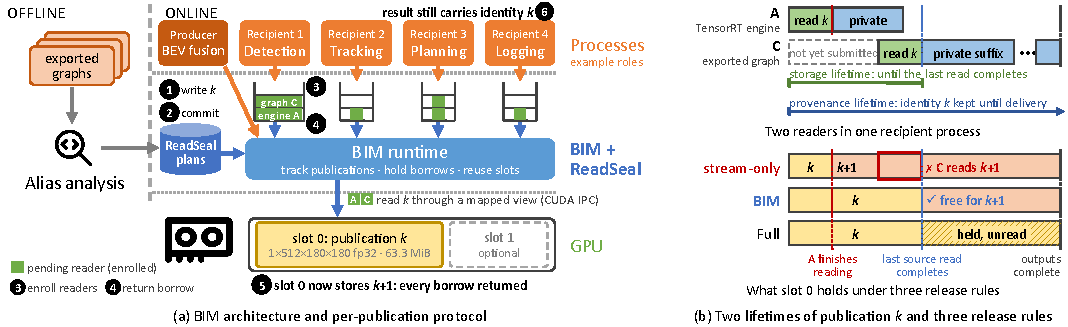
\includegraphics{figures/fig1_overview.pdf}
\caption{\textbf{BIM at a glance.} (a)~Offline, ReadSeal analyzes each exported model graph into a plan. Online, the producer writes frame~$k$ into a slot and commits it (\circled{1}, \circled{2}); each recipient enrolls its readers before they submit GPU work (\circled{3}) and returns its borrow once their source reads complete (\circled{4}); the producer may overwrite the slot after every borrow is returned (\circled{5}), while results still carry identity~$k$ (\circled{6}). (b)~Time runs left to right; TensorRT engine~A and exported graph~C are the readers of the last recipient holding a borrow. Stream-only release lets $k{+}1$ overwrite the slot before the graph reads it; full retention holds the slot until the outputs complete; BIM frees it at the last source read.}
\label{fig:overview}
\end{figure*}

The two obvious answers fail (Section~\ref{sec:motivation}). \emph{Stream-only release} reuses the slot once all GPU work submitted so far has finished. A recipient that has not yet submitted its reads, such as one still waiting in its queue, then silently computes on the next frame: a detector reports objects seen in frame $k{+}1$ under the timestamp of frame $k$, and at 20\Hz{} a vehicle driving at 20\,m/s moves a full meter between the two. \emph{Full retention} holds the slot until every result is ready, as reference-counted zero-copy transports do when each recipient keeps its reference until done~\cite{iceoryx,agnocast}. It is safe, but a frame that finds the slot held is dropped: at 20\Hz, full retention drops every other frame while the recipients sit idle (Fig.~\ref{fig:trace}). Releasing at a hand-placed point after the last read avoids both failures, but only until a model edit moves that read.

\textbf{Key insight.} A shared tensor, the \emph{source}, has two lifetimes (Fig.~\ref{fig:overview}b). Its \emph{storage lifetime} ends when the last operation that reads it completes; its \emph{provenance lifetime} lasts until every result computed from it is delivered, because those results carry the frame's identity. The two can differ widely: in the TransFusion detection head that reads our BEV map, only the first of 287 operations reads it. Later operations use intermediate results in private storage, so they can continue after the shared input is overwritten. A library loan works the same way: a student returns the book once she has read it, although her essay still cites that edition. Like her loan, each recipient's \emph{borrow} on the slot lasts only while it may still read the source. Ending the borrow at the last read lets the slot take the next frame while the previous frame's computation continues.

Ending the borrow at the last read is safe only if three questions have answers. (1)~Which operation reads last? \emph{Views}, tensors that share the input's storage, extend its reads, and one model edit can move this \emph{read boundary} from the first operation to the second-to-last (Fig.~\ref{fig:boundaries}). (2)~Who may still read? A reader that has not yet submitted GPU work leaves nothing to wait on. (3)~Is the analyzed program the one that runs? A boundary derived for one model version can be wrong for the next.

We present BEV-in-Memory (BIM), a middleware contract built on this distinction, and ReadSeal, its mechanism for answering the three questions. BIM keeps apart a frame's identity, a recipient's view of its bytes, and the recipient's borrow of the slot, and registers every recipient's borrow when a frame is published, before any recipient starts (Section~\ref{sec:bim}). ReadSeal answers the three questions in turn: it derives each read boundary by alias analysis of the model graph, enrolls each recipient's readers before they submit work (\emph{enrollment}), and binds each plan to the code, model state, and input layout that execute (\emph{binding}; Section~\ref{sec:readseal}).

The throughput benefit comes from ending the borrow at the last source read; a carefully maintained hand-placed boundary obtains the same benefit. ReadSeal automates that maintenance: it derives the boundary from each model version and rejects execution when the code, model state, or input no longer matches the plan. Our A100 evaluation separates these contributions by measuring delivery under load, then testing boundary derivation and checks under model changes. Our contributions are:
\begin{itemize}
\item \textbf{The two-lifetime view of a shared GPU tensor} (Section~\ref{sec:motivation}). It explains two failures, a silent wrong-frame read caused by composing two correct mechanisms (stream-ordered reuse and GPU events) and the GPU that full retention leaves idle, and shows that release rules are also admission policies, deciding which frames enter the pipeline.
\item \textbf{BIM and ReadSeal} (Sections~\ref{sec:bim}--\ref{sec:readseal}), a cross-process borrowing protocol and graph analysis that derive each last-read boundary, register pending readers, and check that the analyzed program matches execution.
\item \textbf{A measured account of reuse and admission} (Section~\ref{sec:eval}), connecting slot hold time to timely delivery and queueing latency, together with model-update tests of automatically maintained boundaries.
\end{itemize}

% =====================================================================
\section{Background and Motivation}
\label{sec:motivation}

\begin{figure}[t]
\centering
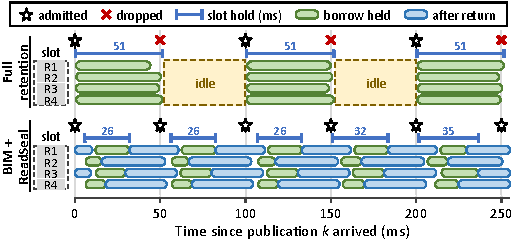
\includegraphics{figures/fig2_trace.pdf}
\caption{\textbf{Full retention refuses frames while the GPU idles.} Measured one-slot trace at 20\Hz{} (repetition~0); R1--R4 are the recipients, and labels give slot hold times in ms. Full's 51\ms{} hold just exceeds the 50\ms{} frame period, so every other frame is refused although the recipients sit idle: full retention is not work-conserving. Under BIM, each recipient's work after its borrow return overlaps the next frame.}
\label{fig:trace}
\end{figure}

\begin{figure}[t]
\centering
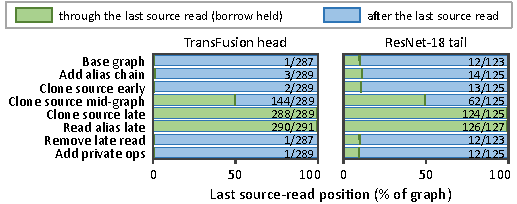
\includegraphics{figures/fig3_boundaries.pdf}
\caption{\textbf{Model edits move the last source read.} Each bar is a graph snapshot; green marks the operations up to and including the last one that may read the shared source, over which the recipient holds its borrow. Each snapshot applies one edit to the base graph (Remove late read undoes Clone source late); labels give the last source-reading operation\,/\,total operations.}
\label{fig:boundaries}
\end{figure}

\textbf{GPU background.} GPU work is asynchronous: a process enqueues \emph{kernels}, the functions the GPU runs, on a \emph{stream}, a queue the GPU executes in order, and moves on. A read is thus over only when its kernel has completed. An \emph{event} is a marker in a stream that completes once the work enqueued before it has finished. PyTorch's \code{record\_stream} lets the caching allocator reuse a buffer only after the work already enqueued on the recorded streams has completed~\cite{recordstream}. CUDA inter-process communication (IPC) lets another process map the same device buffer and wait on shared events. But an event can mark only work already enqueued: no process can wait on reads that another has not yet submitted.

\textbf{Releasing too early fails silently.} The simplest case is a recipient still waiting in its queue. It has enqueued no GPU work, so a rule that waits only for submitted work, such as \code{record\_stream} or a read event, returns the slot once the other recipients' reads complete. The producer writes $k{+}1$, and the waiting recipient later computes a numerically valid result on it while its request still names $k$. No crash or error signals the failure, so a downstream planner has no reason to distrust the result. The same gap can open inside a recipient that combines a TensorRT engine with a framework graph. In our running example (Fig.~\ref{fig:overview}b), the two \emph{readers} are TensorRT engine~A, which signals an input-consumed event after reading its input~\cite{tensorrt}, and exported graph~C. An adapter forwards a view to the graph without reading the source itself. Once the engine's event completes, stream-only release returns the slot although the graph has not submitted its reads. Section~\ref{sec:eval-safety} tests this ordering. ROS~2's CUDA buffer backend exposes the same choice: a subscriber's read handle records a read event when destroyed, and the block is recycled once every handle is released~\cite{cudabackend}; destroying the handle after the engine's read is stream-only release, and holding it until the outputs complete is full retention.

\textbf{Releasing too late wastes the GPU.} Full retention's 51\ms{} hold exceeds the 50\ms{} period at 20\Hz, so every other frame is refused while the GPU idles (Fig.~\ref{fig:trace}). Section~\ref{sec:eval-slots} compares early reuse with adding a second slot.

\textbf{Hand-placed read boundaries go stale.} The read boundary depends on the recipient's whole graph: a view can carry a source read into later operations (Fig.~\ref{fig:boundaries}). In our model-update tests, 14 constructed graph edits, a batch-normalization folding, and a public model substitution move 13 boundaries across 16 transitions (Section~\ref{sec:eval-safety}). A hand-placed boundary must follow these changes to avoid a wrong-frame read. Table~\ref{tab:options} summarizes the options. BIM tracks every recipient before any runs, and ReadSeal derives and checks the boundary against the executing program.

\begin{table}[t]
\caption{Release options for four recipients of one BEV source ($K$: cap on outstanding recipient requests). $^\dagger$Silently, unless digests are refreshed by hand; ReadSeal rejects a stale plan. $^\ddagger$Misses readers that have not yet submitted work.}
\label{tab:options}
\centering
\footnotesize
\setlength{\tabcolsep}{1.8pt}
\begin{tabular}{@{}lllll@{}}
\toprule
\hd{Policy} & \hd{Extra\\memory} & \hd{Slot reusable\\after} & \hd{Read\\boundary} & \hd{Wrong\\frame?} \\
\midrule
Stream-only            & ---      & submitted reads & stream idle & possible$^\ddagger$ \\
Full retention         & ---      & all outputs     & ---         & no      \\
Full, 2 slots, $K{=}8$ & one slot & all outputs     & ---         & no      \\
Clone-on-accept        & 256\,MiB & all copies      & fixed       & no      \\
Manual                 & ---      & all last reads  & by hand     & if stale$^\dagger$ \\
\rowcolor{bimrow}
BIM + ReadSeal         & ---      & all last reads  & derived     & no \\
\bottomrule
\end{tabular}
\end{table}

% =====================================================================
\section{BIM: A Publication-Aware Contract}
\label{sec:bim}

BIM keeps apart three things that zero-copy sharing usually conflates: memory, identity, and permission to read. A \emph{slot} is memory: one of $N$ reusable GPU buffers in the producer's pool on one machine. A \emph{publication} is one frame's tensor written into a slot, with an identity that every result computed from it carries; the same slot holds publication~$k$ and later $k{+}1$. Its tensor, as recipients read it, is the \emph{source}. A \emph{recipient} is a process with one or more \emph{readers}, such as engine~A and graph~C, which access the source through a \emph{view} that fixes how its bytes are interpreted. A recipient's \emph{borrow} is its permission to read the slot, held until none of its readers, running or not yet submitted, can still read the source. Borrows decide when memory is reused; identities decide how results are labeled.

\textbf{Descriptors and views.} Recipients receive small descriptors over a control plane such as ROS~2 and map the resident tensor through a backend, here CUDA IPC via PyTorch's tensor-sharing reductions~\cite{torchmp}. A descriptor carries a publication identity (producer instance and sequence number), a storage locator, and an interpretation: element type, shape, strides, and a checked view range. The view specifies which bytes a recipient may address; the identity specifies which frame those bytes belong to. BIM rejects stale identities and incompatible interpretations.

\textbf{Borrow bits and admission.} A process-shared lock protects slot reservation, the publication sequence, and one borrow bit per recipient, set while that recipient may still read the slot. An arriving frame takes a slot whose bits are all clear or, if none is free, is dropped, not blocked. Once the frame is written, the producer \emph{commits} the publication: it sets every recipient's bit before sending any descriptor, so a recipient is covered even while it waits in its queue. A recipient clears its bit when it returns its borrow; clearing the last bit makes the slot available again without freeing or unmapping it. If publication~$k$ is committed at time~$c_k$ and recipient~$j$ returns its borrow at time~$t_{j,k}$, the slot is held for $H_k$, and with one slot a frame arriving at time~$a$ is admitted only if
\begin{equation}
a\;\ge\; c_k+H_k, \qquad H_k=\max_j t_{j,k}-c_k. \label{eq:hold}
\end{equation} The release rule therefore also decides admission: full retention sets $t_{j,k}$ to the time $j$'s outputs complete, and ReadSeal to the time $j$'s last source read completes (Section~\ref{sec:enroll}). An optional cap~$K$ bounds outstanding recipient requests, each counted from admission to receipt at the output sink. Admission thus has two gates, a free slot and the cap: under overload, BIM refuses frames rather than overwrite a slot that may still be read. ReadSeal enrolls the readers inside each recipient and decides where each borrow ends.

% =====================================================================
\section{ReadSeal: Checked Borrowing}
\label{sec:readseal}

ReadSeal works in two phases (Algorithm~\ref{alg:readseal}). Offline, once per model version, it turns each graph a recipient runs into a \emph{plan} with one part per question of Section~\ref{sec:intro}. The first splits the graph at its read boundary into a \emph{source-reading prefix}, ending with the last operation that may read the source, and a \emph{private suffix}, which computes the rest of the frame's results without reading the shared storage (Section~\ref{sec:derive}). The second lists the \emph{readers} to enroll, the components inside the recipient that read the source, such as engine~A and graph~C (Section~\ref{sec:enroll}). The third holds \emph{binding tokens}, identifiers of the code, model state, and input layout the plan was derived for (Section~\ref{sec:bind}). Online, an \emph{invocation} is one run of a plan on one publication; its recipient may return its borrow only after every operation that may read the source has completed or was cancelled before starting.

\subsection{Deriving the Read Boundary}
\label{sec:derive}

\begin{algorithm}[t]
\caption{BIM's commit and ReadSeal's plan and invocation}
\label{alg:readseal}
\footnotesize
\begin{algorithmic}[1]
\Procedure{Publish}{frame $k$}\Comment{producer (BIM)}
\State \textbf{if} no slot is free or $K$ requests are outstanding, \textbf{drop} $k$
\State write $k$ into a free slot $s$; \emph{commit}: set $b_{s,j}$ for all $j$
\State send each recipient a descriptor of $(k,s)$
\EndProcedure
\Procedure{BuildPlan}{graph $G$}\Comment{offline, per model version}
\State compute $Q_r$ by \eqref{eq:reads} and $\beta$ by \eqref{eq:boundary}
\State split $G$ at $\beta$; record readers $U$ and tokens $T$
\EndProcedure
\Procedure{Invoke}{plan, publication $k$}\Comment{recipient $j$}
\State check $T$; keep identity $k$ for every output
\State enroll every reader in $U$, before any submits GPU work
\State submit the stages in declared order, checking $T$ at each entry
\State \textbf{on} failed check: cancel unsubmitted reads, drain, publish nothing
\State \textbf{on} each completed or cancelled read: \textbf{if} \eqref{eq:return} holds, clear $b_{s,j}$
\State \textbf{on} completed outputs: publish them with identity $k$
\EndProcedure
\end{algorithmic}
\end{algorithm}

The analysis runs on each graph, a fixed-shape, functional directed acyclic graph (DAG) of operations. Of the two lifetimes, only storage needs analysis. Every result carries the frame identity attached at acceptance. Storage sharing propagates through views: a slice of the source is a view, so an operation on the slice still reads the source, whereas a convolution reads the source but writes fresh storage, so operations on its output do not. In our running example, the adapter only forwards a view; the graph receiving that view reads the source.

Formally, let $S(v)$ be the set of shared roots whose storage a value~$v$ may alias, with $S(r)=\{r\}$ for the source~$r$. For an operation~$o$ with inputs $v_i$ and output $v_o$, let $\mathcal{A}_o$ index the inputs the output may alias and $\mathcal{R}_o$ the inputs $o$ reads. Then
\begin{equation}
\begin{aligned}
S(v_o)&=\textstyle\bigcup_{i\in \mathcal{A}_o} S(v_i),\\
Q_r&=\{\, o : \exists\, i\in \mathcal{R}_o,\; r\in S(v_i) \,\},
\end{aligned}\label{eq:reads}
\end{equation}
where $Q_r$ is the set of operations that may read the source. With the operations numbered $o_1,\dots,o_n$ in execution order, the read boundary is the position of the last one in $Q_r$,
\begin{equation}
\beta=\max\{\, i : o_i\in Q_r \,\}, \label{eq:boundary}
\end{equation}
so the source-reading prefix is $o_1,\dots,o_\beta$ and the private suffix $o_{\beta+1},\dots,o_n$. Fig.~\ref{fig:boundaries} labels each graph snapshot with $\beta/n$; the base head has $\beta=1$ and $n=287$.

Operator summaries cover 42 reviewed operator variants in ATen, PyTorch's operator library, plus selection of a tuple element at a fixed index. Each summary counts every operand as read and treats an output as sharing storage whenever the operator's declared signature permits aliasing with an input. Plan construction rejects unsupported mutation, opaque callbacks, and source views that escape the graph. The implementation compiles the prefix and suffix into separate executable stages. A CUDA event after the prefix then marks completion of all its source reads.

\subsection{Enrolling Readers Before Submission}
\label{sec:enroll}

Registration happens at two levels. BIM registers recipients: its commit sets one borrow bit per recipient (Section~\ref{sec:bim}). ReadSeal registers the readers inside a recipient: when it accepts an invocation, it enrolls every reader in the plan at once, before any of them submits GPU work. Each reader~$u$ marks the end of its source reads with one completion event, A's input-consumed event or the event recorded after C's prefix. Let $U_j$ be the readers of recipient~$j$. Then $j$ returns its borrow for publication~$k$ at the first moment when
\begin{equation}
\forall u\in U_j:\quad \mathit{done}_u \lor \mathit{cancelled}_u, \label{eq:return}
\end{equation}
where $\mathit{done}_u$ holds once $u$'s completion event has completed and $\mathit{cancelled}_u$ once $u$ has been cancelled before submission. The condition ranges over every enrolled reader, not only those with work in flight: when A's event completes, C's read is still pending, so the bit stays set although C has enqueued no GPU work. Returning the borrow clears only $j$'s bit; the slot takes the next publication once every recipient has returned its borrow, while $j$'s private suffix keeps computing results that carry identity~$k$. Enrollment prevents the wrong-frame read of Section~\ref{sec:motivation}; the analysis sets how early the borrow ends.

% Fig. 5 is defined here, inside Section IV (page 4), so that it floats to the top of the page where Section V starts.
% ---------------------------------------------------------------------
\begin{figure*}[t]
\centering
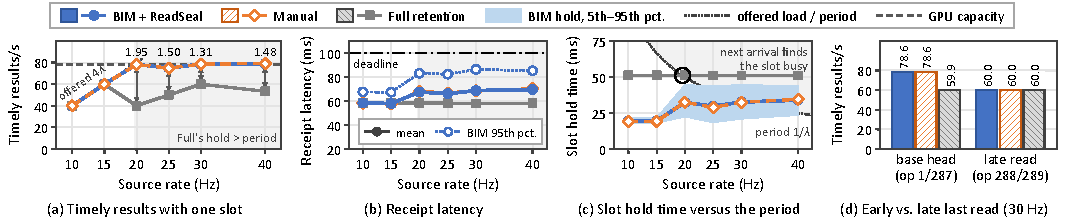
\includegraphics{figures/fig5_delivery.pdf}
\caption{\textbf{Early reuse raises one-slot delivery under load, with a latency cost.} One slot, no pipeline-wide cap~$K$; six runs per condition and policy. Each input frame offers four recipient results; results/s counts individual results. (a)~Labels give BIM/Full ratios. (b)~Mean receipt latency; BIM's 95th percentile is computed per run and averaged. (c)~Mean hold and BIM's 5th--95th percentile; shading marks where Full's hold exceeds the frame period. (d)~Moving the last read to the graph's end removes the gain.}
\label{fig:delivery}
\end{figure*}

\subsection{Binding Plans to Execution}
\label{sec:bind}

At construction, ReadSeal captures the functions to run, clones model tensors, and records binding tokens~$T$: identifiers and metadata for code and globals, model storage and version, input layout, and the compiled stages. Acceptance and each stage entry compare $T$ with the corresponding values of what is about to run, $\hat T$, and proceed only if $\hat T=T$ (Algorithm~\ref{alg:readseal}). A failed check cancels unsubmitted reads, drains started work, and publishes nothing. The application supplies the exported graph, the completion event that marks each native engine's last input read, and the component and output dependencies; new operators require reviewed summaries.

\subsection{Correctness Conditions}
\label{sec:correctness}

The analysis must include every operation that can read the source. It assumes that operator summaries conservatively describe reads and storage sharing, kernels obey those summaries, and the graph executes in the analyzed order.

\begin{proposition}
Under these assumptions, $Q_r$ in Eq.~\eqref{eq:reads} contains every operation that can read the shared source. No operation after the derived boundary $\beta$ reads that source.
\end{proposition}

\begin{proof}[Proof sketch]
Initially $S(r)=\{r\}$. At each operation, the union in Eq.~\eqref{eq:reads} preserves the shared roots of every input that its output may alias. Induction over graph order therefore includes every source alias in the corresponding $S(v)$. The read rule places every operation consuming such storage in $Q_r$; by Eq.~\eqref{eq:boundary}, none follows $o_\beta$.
\end{proof}

For the runtime, each reader's completion event must occur after its source reads, mappings must remain valid, and identities must remain unique while referenced. Algorithm~\ref{alg:readseal} registers every reader before submission, checks the plan at execution, and returns a borrow only when Eq.~\eqref{eq:return} holds. BIM permits overwrite after all recipient bits clear. Together, these steps preserve the source until every reader finishes, while results keep the identity captured at acceptance.

% =====================================================================
\section{Evaluation}
\label{sec:eval}

% The slots figure is defined at the start of Section V so that it floats to the page after the delivery figure.
\begin{figure*}[t]
\centering
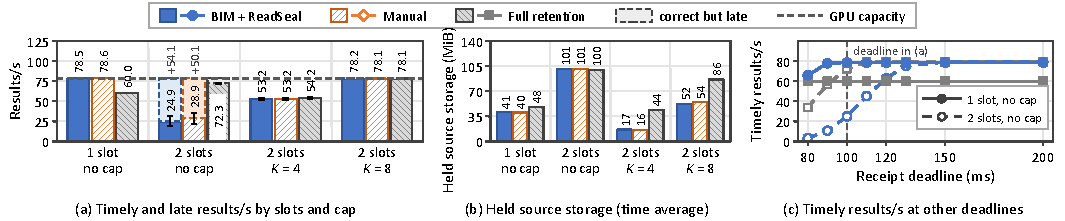
\includegraphics{figures/fig6_slots.pdf}
\caption{\textbf{One BIM slot matches full retention with two slots and a request cap} (30\Hz; six runs per condition and policy). $K$ counts outstanding recipient requests; eight requests are two full groups of four. (a)~Solid: timely results; dashed: correct but late; whiskers: 95\% intervals. (b)~Time-averaged source storage held by unreturned borrows, not allocated memory. Device peaks are 5,078\MiB{} with one slot and 5,142\MiB{} with two for every policy. (c)~BIM and Full re-scored at different deadlines using the same runs.}
\label{fig:slots}
\end{figure*}



The evaluation answers five questions in turn: when early reuse pays and what it costs in latency (Section~\ref{sec:eval-delivery}, Fig.~\ref{fig:delivery}); whether a second slot could do the same (Section~\ref{sec:eval-slots}, Fig.~\ref{fig:slots}); how jitter, mixed recipients, and copying change the picture (Section~\ref{sec:eval-mixed}, Fig.~\ref{fig:mixed}); whether BIM stays safe under reordering and model change (Section~\ref{sec:eval-safety}); and what ReadSeal's checks cost (Section~\ref{sec:eval-cost}).

\subsection{Setup}
\label{sec:eval-setup}

\textbf{Scope and platform.} We evaluate cross-process reuse of saved BEV features on one NVIDIA A100 PCIe 40\,GB GPU. The producer, four recipients, and output sink communicate through multiprocessing queues and share storage and events through CUDA IPC. This setup measures reuse and admission independently of feature extraction; it does not run ROS~2, the BEV front end, or an embedded driving stack. The runtime uses PyTorch 2.1.2, CUDA 12.1, and TensorRT 10.3. Without NVIDIA's Multi-Process Service (MPS), recipient kernels take turns on the GPU. Records, validators, campaign details, and analysis scripts are public.\footnote{\url{\artifacturl}.}

\textbf{Workload.} The exported graph (C) is BEVFusion's functional TransFusion head~\cite{bevfusion,transfusion}, with 287 operations. The producer publishes precomputed 63.3\MiB{} feature maps from three fixed nuScenes-mini frames~\cite{nuscenes}. The native engine (A) runs the head's shared convolution, ReLU, and global average pooling in TensorRT; an adapter forwards a view to the graph. This controlled composition gives each recipient two readers of the same source, each with its own completion event. Four recipients run identical compositions in the rate and slot sweeps; Section~\ref{sec:eval-mixed} varies their components. A pretrained ResNet-18 tail, comprising residual stages and classifier with saved stem activations as the shared source, serves in the correctness, model-change, and cost tests.

\textbf{Policies.} All policies share the pool, workloads, queues, and admission settings. BIM uses ReadSeal; \emph{Full} retains the source until its outputs complete. The hand-placed baseline has two implementations: \emph{Manual}, used in the rate and slot sweeps, independently enrolls both readers and checks hand-maintained code and model digests; \emph{Manual-checked}, used in the jitter and mixed-recipient tests, uses BIM's runtime and binding checks with a hand-placed boundary. \emph{Clone-on-accept} gives each recipient a private copy when it accepts a request.

\textbf{Metrics.} The source publishes frames at rate~$\lambda$, in Hz. Each published frame offers one \emph{result}, the output delivered by one recipient, to each of four recipients; offered load is therefore $4\lambda$ results/s. A result is \emph{timely} if it reaches the sink after device-to-host transfer and IPC, passes source-identity and reference-output checks, and arrives within 100\ms{} of the frame's planned arrival. Late results and refused frames are counted separately. \emph{Receipt latency} runs from planned arrival to sink receipt; \emph{slot hold time} runs from commit to the last borrow return. Section~\ref{sec:eval-mixed} additionally measures complete frames: all four intended results must be correct and timely, with every scheduled frame in the denominator.

\textbf{Queue settings.} The rate and slot sweeps permit at most two pending requests and four in flight per recipient. Optional cap~$K$ limits outstanding recipient requests across the pipeline; $K{=}8$ accommodates two full groups of four requests. \emph{No pipeline-wide cap} leaves the per-recipient queue limits in place.

\textbf{Statistics.} Rate and slot runs have 2\,s of warm-up, 12\,s of measured arrivals, and a complete drain. Condition and method order are randomized, with six paired repetitions per condition; brackets give pointwise 95\% intervals from 20,000 paired whole-run bootstrap draws. The two campaigns in Section~\ref{sec:eval-mixed} use queues of eight, 10\,s of warm-up, and 30\,s of measurement, with six paired runs and pointwise 95\% $t$ intervals. Campaigns are analyzed separately. Latency summaries describe individual recipient results in the rate sweep (mean and per-run 95th percentile) and complete correct frames in the mixed-recipient study (per-run 99th percentile).

\subsection{Early Reuse Raises Delivery Under Load}
\label{sec:eval-delivery}

Once the frame period falls below full retention's slot hold time, early reuse delivers more (Fig.~\ref{fig:delivery}a). All policies deliver the offered 40 and 60 results/s at 10 and 15\Hz. At 20\Hz, BIM delivers 78.3 results/s and Full 40.1, a paired difference of 38.2 [37.9, 38.5]; at 25--40\Hz, BIM delivers 1.31--1.50$\times$ as many. BIM stays within 0.2 results/s of Manual at every rate.

\textbf{Why the gap opens.} The four recipients take turns on the GPU, so each takes 48--49\ms{} from acceptance to output, against about 11\ms{} in isolation (Section~\ref{sec:eval-cost}), and the pipeline completes about four results per 51\ms, 78.4 results/s (Fig.~\ref{fig:delivery}a, dashed). Full's hold spans nearly this whole time, $H_k=51$\ms{} at every rate (Fig.~\ref{fig:delivery}c), so by Eq.~\eqref{eq:hold} it refuses the next frame exactly when frames arrive faster than the GPU can finish them: Full admits every other frame at 20\Hz{} and every third at 40\Hz, and the GPU idles in between (Fig.~\ref{fig:trace}). BIM's hold ends at the last recipient's enrolled reads. In the base head these are the first operations, yet the hold lasts 30--34\ms{} under contention, because the last recipient must wait its turn on the GPU before they run: a read's position in the graph is not its share of the time. The hold still fits the period at 20\Hz, where BIM refuses only 2\% of frames, and BIM reaches the ceiling at 20, 30, and 40\Hz. At 25\Hz, periodic arrivals lock it into admitting three frames in four (75.0 results/s), since a refused frame is replaced only one 40\ms{} period later. The 1.95$\times$ peak arises because Full's hold barely exceeds the period at 20\Hz; 1.31--1.50$\times$ at 25--40\Hz{} is the sustained gain.

\textbf{Latency cost.} Early reuse changes admission, not model speed, so the extra results queue behind GPU work (Fig.~\ref{fig:delivery}b): BIM's mean receipt latency at 20--40\Hz{} is 66--70\ms, 8--11\ms{} above Full's, and its per-run 95th percentile averages 82--86\ms{} against Full's 67\ms. Re-scored at 100--200\ms{} deadlines, one-slot BIM's lead at 30\Hz{} is unchanged; at a tight 80\ms{} it narrows from 18.5 to 5.9 results/s (Fig.~\ref{fig:slots}c).

\textbf{The gain requires a private suffix.}\label{sec:eval-late} In the late-read test at 30\Hz, the base head gives BIM 78.6 results/s and Full 59.9; with the last source read at operation 288 of 289 (Fig.~\ref{fig:boundaries}'s late clone), all three policies deliver 60.0 (Fig.~\ref{fig:delivery}d), because BIM's hold rises from 32.7 to 51.7\ms{} and leaves nothing to overlap.

\subsection{One Slot Matches Two, and Two Need a Cap}
\label{sec:eval-slots}

We first compare one-slot early reuse with a larger pool, then vary admission within that pool (Fig.~\ref{fig:slots}a). At 30\Hz, one-slot BIM delivers 78.5 results/s and one-slot Full 60.0. Adding a second slot raises Full to 72.3 results/s without a pipeline-wide cap; setting $K{=}8$, enough for two full groups of recipient requests, raises it to 78.1. A tighter cap of $K{=}4$ yields 54.2. Thus one-slot BIM reaches the measured capacity with 64\MiB{} less device peak than two-slot Full.

\textbf{A release rule is also an admission policy.} By Eq.~\eqref{eq:hold}, a slot pool acts as an admission controller: one slot paces BIM to the GPU by itself, admitting about two thirds of the results offered at 30\Hz. Two uncapped slots let BIM admit frames that the GPU cannot start in time; they wait in the recipients' queues and miss the deadline. Uncapped two-slot BIM admits about as many results as one-slot BIM, all correct, but only 24.9 per second are timely, against 72.3 for Full, whose long hold still throttles admission: the time from a frame's arrival to the start of its processing rises from about 29\ms{} under Full to 54\ms. For BIM, already at the GPU's ceiling, the second slot buys only queueing delay, as in bufferbloat, where oversized network buffers add delay without adding throughput. Manual likewise collapses (28.9), and at a 150\ms{} deadline uncapped BIM and Full both deliver about 79 results/s (Fig.~\ref{fig:slots}c).

\textbf{An explicit cap separates admission from safety.} At $K{=}8$, BIM, Manual, and Full all deliver 78.1--78.2 results/s. In the two-slot rate sweep at 20--40\Hz, uncapped BIM delivers 20--40 results/s and Full 71--72, whereas both deliver 78.0--78.3 at $K{=}8$. Held source storage at $K{=}8$ (Fig.~\ref{fig:slots}b) falls from 86.4\MiB{} under Full to 52.3\MiB{} under BIM at an unchanged device peak. This measures how much source storage is still unavailable for reuse, averaged over time. ReadSeal decides when reuse is safe; the admission cap controls queueing.

\subsection{Jitter, Mixed Recipients, and Copying}
\label{sec:eval-mixed}

\begin{figure}[t]
\centering
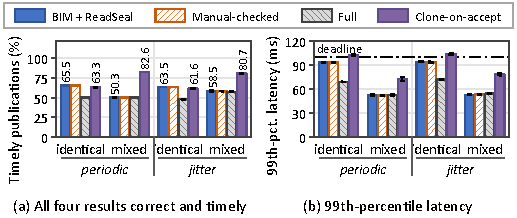
\includegraphics{figures/fig7_mixed.pdf}
\caption{\textbf{Jitter keeps the gain; with mixed recipients, one reading late, copying wins} (30\Hz, one slot, no pipeline-wide cap; 6 runs per bar; whiskers: 95\% $t$ intervals). (a)~Share of the 900 publications per run whose four results are all correct and timely; (b)~per-run 99th-percentile latency of publications whose four results are all correct. \emph{Identical}: four copies of the composition; \emph{mixed}: four different recipients, one reading late.}
\label{fig:mixed}
\end{figure}

The next study tests whether every intended recipient completes on time, using the complete-frame metric in Fig.~\ref{fig:mixed}. At 30\Hz{} with one slot and no pipeline-wide cap, arrivals are periodic or displaced by up to 0.8 of a period (\emph{jitter}). Recipients are either \emph{identical} copies of the composition or \emph{mixed}: the native engine alone, the exported head alone, their composition, and a composition that reads the source late. Manual-checked supplies the hand-placed comparison in this study.

\textbf{Jitter keeps the gain.} With identical recipients, BIM completes 65.5\% of publications with periodic arrivals and 63.5\% with jitter, near the two thirds the shared GPU can finish, against Full's 50.0\% and 48.0\%. With mixed recipients the slot is held until the late reader's last read, and BIM completes 50.3\% (58.5\% with jitter), under one point above Full.

\textbf{Copying wins when recipients read late.} Clone-on-accept frees its slot once the copies are made: with mixed recipients it completes 81--83\% of publications, 22--32 points more than BIM, at a 256\MiB{} higher device-memory peak and 20--25\ms{} more 99th-percentile latency; with identical recipients it completes about 2 points fewer. A separate 168-run rate sweep with identical recipients isolates the late read: cloning stays within 3 results/s of BIM at every rate but leads by 16.4 (1.27$\times$) when every recipient reads late. Manual-checked stays within 0.13 percentage points of BIM everywhere, including 12 all-late runs: the gain comes from where the borrow ends, not from how that point is found.

\subsection{Safety Across Reordering and Model Changes}
\label{sec:eval-safety}

\textbf{Future readers.} In six controlled ordered tests, the exported graph's outputs under stream-only release matched the replacement frame; BIM's and Manual's matched the admitted frame. The graph had not yet submitted its reads when the engine completed, so recording stream use did not cover those later reads~\cite{recordstream}. Separately, in the 144 rate and late-read runs, all 109,592 results delivered by BIM, Manual, and Full carried their admitted identity and matched reference outputs.

\textbf{Boundaries under model change.} Fig.~\ref{fig:boundaries} shows derived boundaries for sample snapshots; ResNet's residual connection already needs a later boundary than the head's. Across eight snapshots per model, three inputs, and two methods, all 96 ordered-overwrite cases (540 output tensors) matched unsplit references after the regenerated boundary, and binding validation rejected all 22 attempted substitutions of plan, code, globals, model state, or input before the affected stage.

\textbf{Maintenance.} We replay 16 transitions (14 constructed graph edits, one batch-normalization folding, and a public ResNet-18 to ResNet-50 substitution) that move 13 read boundaries. Manual must update each by hand and refresh 16 digests even to detect a stale boundary, which otherwise fails silently; ReadSeal re-derives every boundary, without annotations, in 0.08--0.21\,s of CPU time per plan. Its checks also catch stale hand-placed boundaries: in the jitter and mixed-recipient tests, a Manual-checked boundary made stale by an added late read was rejected until moved, and all 24 update cases gave exact outputs.

\subsection{Execution Cost and Coverage}
\label{sec:eval-cost}

An isolated-process test times recipient acceptance to output publication (8 process repetitions of 50 randomized invocations per method; three inputs; base and late variants of both models). ReadSeal's checks add 0.8--0.9\ms{} per invocation, mostly at acceptance and stage submission: 8\% over Manual for the base head (11.8\ms{} against 10.9\ms) and 22--23\% for the lighter ResNet tail. In the pipelines above, this cost overlaps shared GPU work; even at 10 and 15\Hz, BIM's mean receipt latency is within 0.4\ms{} of Manual's. A static survey of 14 torchvision tails with untrained weights accepts nine, with boundaries in their first 1--12 operations, and rejects five for unsupported operators.

% =====================================================================
\section{Discussion}
\label{sec:discussion}

\textbf{When to use BIM.} The measurements connect source reuse to admission: after early source reads, a single slot can pace arrivals to the shared GPU while private computation continues. ReadSeal maintains this boundary as models change. Larger pools need a request cap when queueing threatens deadlines. For late readers, copying trades memory and tail latency for earlier reuse; full retention remains an option when memory rules out copies. A copy is itself a source read, so queued recipients still need to be registered before the slot can be reused.

\textbf{Portability.} BIM requires cross-process storage mapping and completion events that cover each reader's source access. ROS~2's CUDA buffer read handles~\cite{cudabackend} and NvSciStream's per-consumer packet release~\cite{nvscistream} provide candidate integration points. A port must implement the storage and event adapter and validate its ordering guarantees. Custom operators require reviewed read and alias summaries; native engines supply an event marking their last input read.

\textbf{Deployment.} The prototype runs declared topologies with single-stream stages; a topology change requires a new plan. A crashed recipient leaves its borrow outstanding and prevents slot reuse. Recovery requires confirmation that the recipient's GPU work has stopped before its borrow can be removed.

% =====================================================================
\section{Related Work}
\label{sec:related}

\textbf{Zero-copy robotics middleware.} iceoryx and Agnocast give ROS~2 subscribers direct access to publisher-owned shared memory~\cite{iceoryx,agnocast}. For GPU data, NITROS keeps its zero-copy path within one process~\cite{nitros}, and ROS~2's \code{rosidl::Buffer} moves tensor bytes between processes through CUDA IPC~\cite{rosidlbuffer}. Readers that have not yet submitted, and where to release, are left to the application.

\textbf{Release fences.} Android's BufferQueue lets a consumer release a pooled buffer with a fence while still reading it~\cite{bufferqueue}, and NvSciStream returns a multicast packet to its pool once every consumer has released it~\cite{nvscistream}. BIM's borrow bits implement this protocol; ReadSeal derives where the release fence goes, which these interfaces leave to the application.

\textbf{Last use and safe reclamation.} Compilers and runtimes reuse a buffer after its last use, as in TVM's static memory planning~\cite{tvm}, and Rust's non-lexical lifetimes end a borrow there~\cite{nll}; all see every use in one program, in program order. Safe memory reclamation, such as read-copy-update (RCU) grace periods~\cite{rcu}, reuses memory once no reader can hold it, but protects only readers that have announced themselves. In RCU terms, BIM's commit opens every recipient's read-side section on its behalf, and ReadSeal closes it at the derived last read. ReadSeal's bindings, like PyTorch~2's guards~\cite{pytorch2}, reject execution whose assumptions changed.

% =====================================================================
\section{Conclusion}

BIM separates a shared input's storage lifetime from the identity carried by its results. ReadSeal makes that separation executable: it derives the last-read boundary, registers readers before submission, and checks the plan against the running program. The evaluation shows how safe early reuse improves timely delivery by admitting the next frame while private computation continues, and how model analysis maintains the boundary through updates. The central lesson is that source lifetime is both a correctness condition and an admission decision. Future work will integrate BIM with ROS~2 and automotive sharing backends, measure the checks on embedded cores, and extend the design to concurrent recipients and selective copying for late readers.

\ifaidisclosure
\section*{Acknowledgment}
OpenAI Codex assisted with language editing, readability revisions, figure regeneration from existing source files, and build verification for this revision. The experimental data and figure values are unchanged.
\fi

\bibliographystyle{IEEEtran}
\IEEEtriggeratref{7}
\bibliography{refs}

\end{document}
